\chapter{Design and Implementation}


There are several goals and contributions I want to achieve. One main goal is to be able to recognize asbestos fibers in microscopic images, and show that transfer learning can be done even in this cross-domain specific task. Transfer learning is especially important, since there are only several hundred images to learn from. To achieve this, different CNN architectures are evaluated, with and without transfer learning. Also, in order to achieve better accuracy on the asbestos recognition task, I will alter the current architectures to better meet this specific task's characteristics. Data augmentation with several cropping methods and different combinations of the data set will be iterated over. As already mentioned in the introduction there is no baseline from the laboratory or any research that can be used for comparison. Therefore a new baseline needs to be established with a simple CNN. Also an inter-annotator agreement rate has been computed. In this chapter I explain and discuss the different methods used in this thesis, talk about modifications done on the architectures and dataset.

\section{Problem Description}

The provided dataset consists of about 2'000 microscopic images with and without asbestos fibers. The images come in two different dimensions and different qualities. Most of the images are 1024x768 pixels but some are in 1024x1024 pixels. Only a small subset was pre-labled and the remaining images needed to be labeled by hand, an error-prone task since I was never professionally instructed on how to do it. After labeling the images, some of them were sent back to the laboratory for checking the labeling, but there were many images, that the experts were uncertain on how to label and put them into a new folder which they called  "uncertain". From 441 images I labeled and sent the laboratory for checking 78 images came back as being suspected to contain asbestos but they were not quite sure. That's about 5.65\%. The detection of traces of asbestos by images is indeed very difficult and the error rate increases significantly as stated by the laboratory. In a next step these uncertain samples would be chemically examined to know for sure, which is beyond the scope of this thesis. In Figure \ref{fig:basic_examples} three example images are shown. One with asbestos, one without and one image with an error, that makes it difficult to be used for the training. The first dataset used includes all the images, but in later dataset alterations, these images with errors in them are removed.

\begin{figure}[t]
\centering
\subfigure{
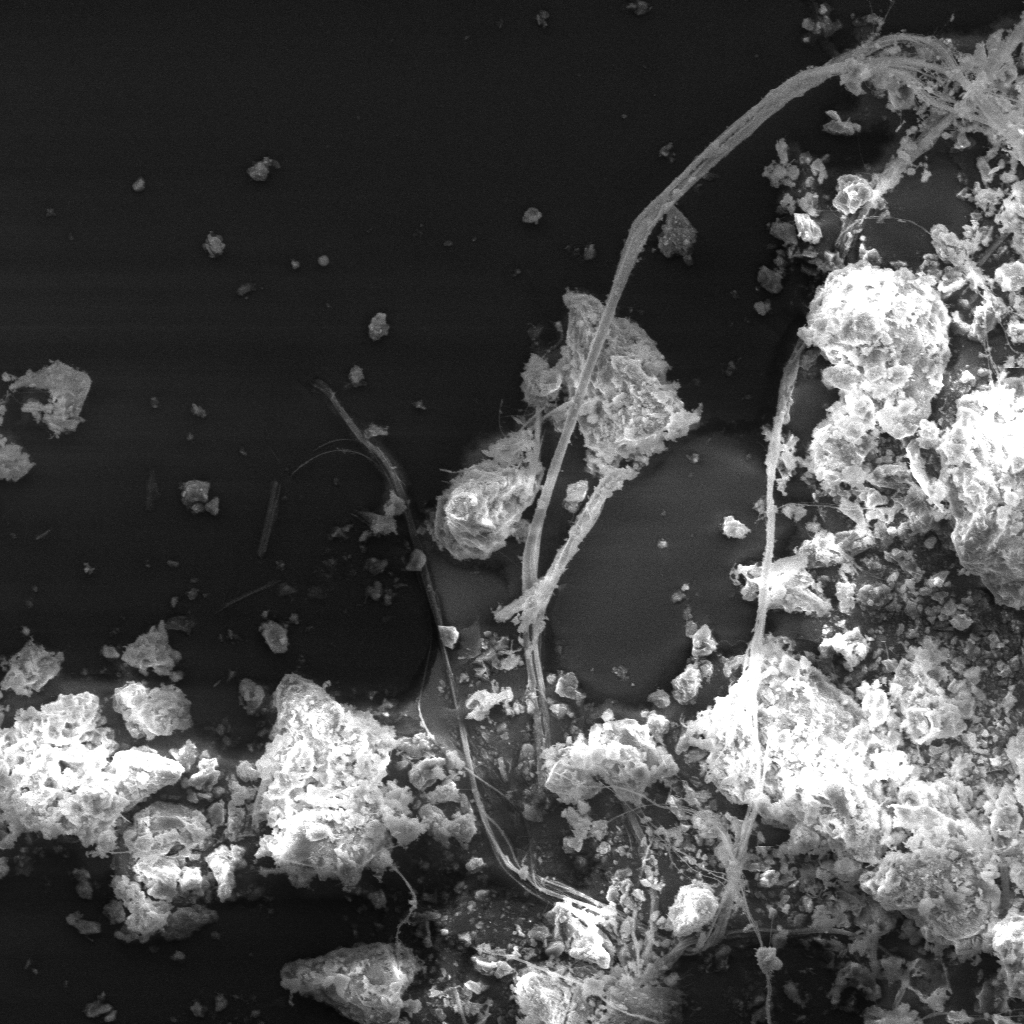
\includegraphics[width=.3\textwidth]{images/chapter4/asbestos.png}
}
\subfigure{
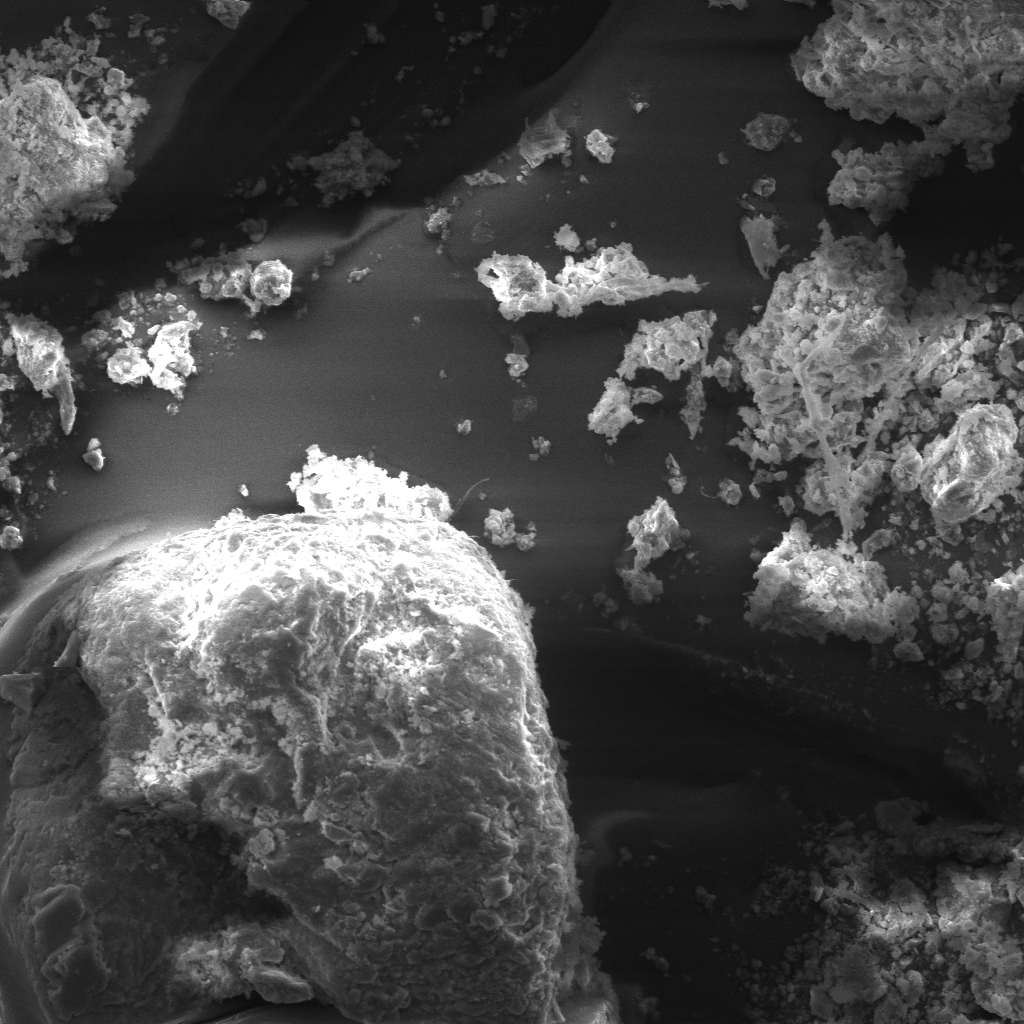
\includegraphics[width=.3\textwidth]{images/chapter4/non-asbestos.png}
}
\subfigure{
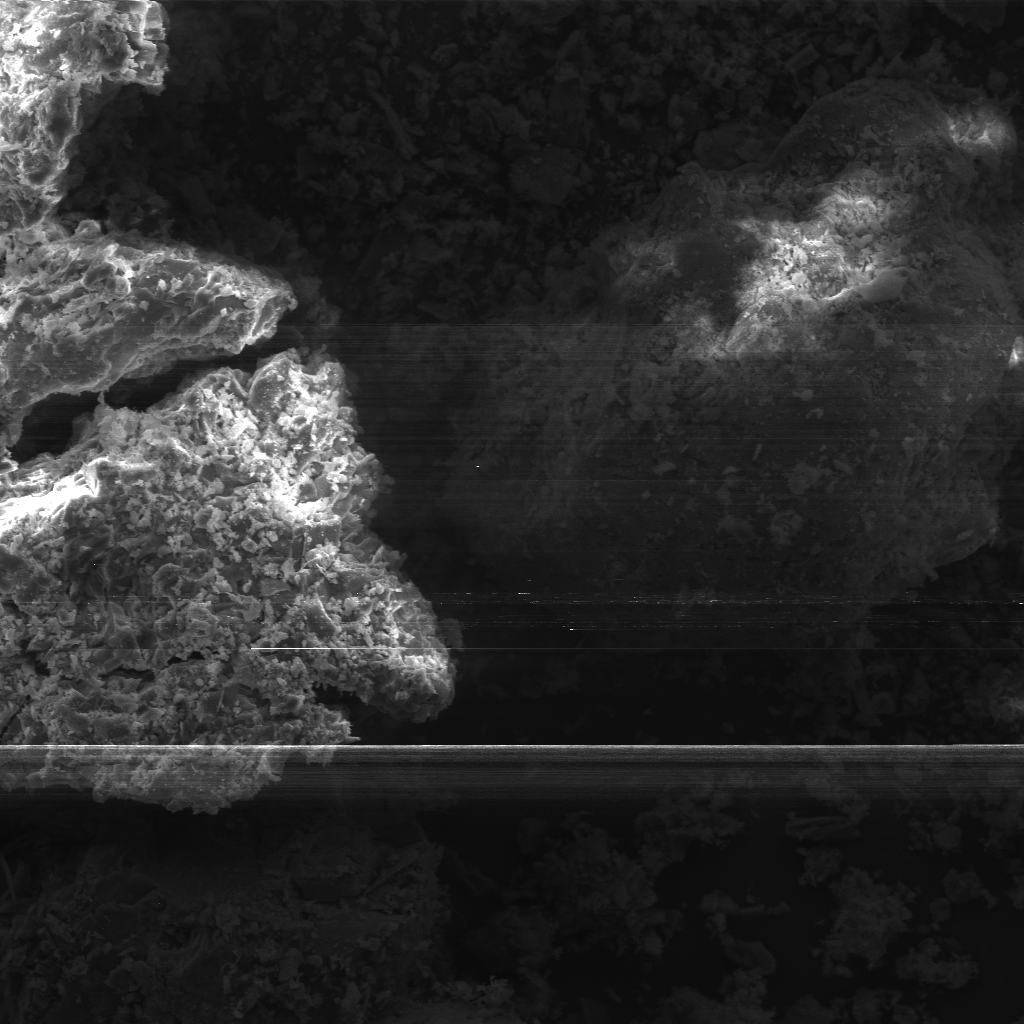
\includegraphics[width=.3\textwidth]{images/chapter4/fail.png}
}
\caption{On the left side the image shows a clear asbestos fiber, in the middle an image without asbestos is shown. On the right side, en example is provided of images that were processed with errors.}
\label{fig:basic_examples}
\end{figure}

\newpage

Since the images are quite large, they will drastically increase in size, once decoded into a PIL object, or Tensor object. On the provided hardware, the memory of four Tesla K80 won't be enough to process whole images during training. Most architectures resize the images to much smaller dimensions ranging from 224x224 for ResNet to 299x299 pixels for Inception v3.

\section{Baseline}

There are two different methods used to acquire a baseline that can show improvements from changes in architectures and provide a better understanding of the data. The first one is to use a very basic CNN with grid search to find the best hyper parameters. This will give a first and low estimation of the accuracy that can be achieved. Also it provides a minimum requirement of this thesis, to improve on that performance. Additionally to the basic CNN, AlexNet will be also evaluated and used as a baseline. For AlexNet I will use both, grid search and SigOpt for finding the best hyperparameters and compare the findings against each other.\\

The other method is the inter-agreement rate or Randolphs' kappa which is a chance-adjusted measure of agreement for any number of classes and raters \cite{randolph2005free}. Randolphs' kappa is a free-marginal kappa that is used when the raters have no fixed number of cases assigned to a specific class as opposed to the traditional Fleiss' kappa, where raters know a priori how many elements a certain class expects. With the asbestos images, this is not the case and the raters have no knowlegde about the asbests versus non-asbestos ratio. Randolph's kappa is an extension of the Fleiss' kappa. For the calculation a online calculator is used \cite{humanlevel2014}.

\section{Data Augmentation}

One common problem in Deep Learning is the amount of data needed to be able to train a model well. This requirement of having huge datasets arises from the need to train an even larger number of parameters of the model, which usually goes into the millions for current state-of-the-art architecuters like VGG's \cite{simonyan2014very}, ResNet's \cite{he2016deep} or Inception \cite{szegedy2015going, szegedy2016rethinking}. Initially the weights for the filters are randomly chosen and then changed during backpropagation in order to lead to a lower loss from the loss function and hopefully lead to a higher generalizability. Having not enough images to train on will lead to a very poor inference through overfitting to the training images. Such a model will not generalize well to unseen data in the test-set even if the architecture has been trained until convergence. Convergence means having trained  for so many epochs, that there is no significant change in the weights from one epoch to another. Many studies have found some correlation between overall performance of the model and its size (number of parameters and layers) with lower layers of the model capturing very basic information like horizontal and vertical lines or color gradients whereas higher layers capturing the overall structure of the object that takes in more of the spatial characteristics. In order to mitigate the problem of overfitting more data is needed. There are only a few hundred good and usable images provided for the asbestos recognition task. They are highly specialized SEM images done in a very specific way including zoom, lightening and position. Finding more images on the internet is impossible so data augmentation is the only viable option to increase the dataset with more images to train on and therefore increase performance. A big dataset is required to be able to generalize the model and perform well on the test-set. Transfer learning might help but the fine-tuning still needs to be done after transferring the weights to the current task and more images allow better fine-tuning. Transfer learning and data augmentation are complementary methods to improve the performance.

Instead of working on the same set of images in every epoch, the images are randomly transformed in such a way, that the label still applies. Therefore every epoch learns with a new variation of the training-set thus reducing overfitting and creating much more images then there are present.

There two main forms of data augmentation. Offline and online augmentation. With offline data augmentation the images are augmented separately and saved to disk. This increases the overall size of the dataset by as many transformations that are done on an image. E.g. flipping horizontally and vertically would result in a three time increase of the dataset. The convolutional neural network would be able to more robustly classify objects in different places and different orientations leading to increased invariance. The downside of offline augmentation is the increase of disk space and therefore disk I/O during training that slows down the learning. With offline data augmentation the training process remains static and there is no randomness included. Adding more epochs would mean to learn more times on the same set of images present on disk.
Online data augmentation happens on the fly and does not need more disk space and disk I/O since it all happens in memory. The image is first loaded into memory and then several transformations are applied to the image. These transformations can be flipping, rotating, scaling, distorting and cropping in different places, and it all is done randomly. Especially the rotating and cropping when done randomly yields new images with every new epoch since the transformation is on a continuous scale. Online augmentation is therefore preferred since it leads to faster learning while reducing overfitting to the training images.

\section{Transfer Learning}

Finding millions of images on the internet of day-to-day objects is an easy task. Finding images on specialized objects like cancer cells in certain tissues is almost impossible. Especially when the equipment with all the settings is also different from hospital to hospital. To mitigate this problem transfer learning can be applied. With this method, the pre-learned weights for a certain architecture can be downloaded from the internet. These weights were obtained learning the model for a long time (until convergence) with a dataset like ImageNet. The hope is that the low and mid layer features are very similar even across problem domains. E.g. a cancer tumor has edges and colors (low-layer features) like any real world object from the ImageNet dataset and might even resemble certain real-life objects (mid-layer features). These layers can be used and fine-tuned to the current task. This gives the model a much better starting point other than initializing all weights of the model randomly and training them from scratch. 

It has been shown that pre-training on ImageNet indeed yields better results through obtaining good general-purpose features in tasks like image classification \cite{sharif2014cnn} and object detection \cite{girshick2014rich, sermanet2013overfeat}. But when the target domain is even farther away like for example human pose estimation \cite{carreira2016human}, image segmentation \cite{dai2016instance} and image captioning \cite{donahue2015long, karpathy2015deep}, pre-training on ImageNet seems to be able to help. Transfer learning has become the de facto standard for solving many different computer vision problems because it promises faster convergence and better accuracies despite the datasets getting bigger and the architectures deeper. Huh et al. \cite{huh2016makes} tried to shed light into this heuristic by examining how various aspects like number of classes, dataset size, ratio of  images per class and fine-grained versus coarse-grained class labels impact the performance of training from scratch versus fine-tuning with pre-trained weights. They found that although pre-training does help in many aspects the commonly held beliefes are not as accurate. For example they conclude that a significant reduction in number of classes or the number of images used in pre-training does not significatnly effect the performance of the transfer task, arguing that deep learning might not be as data-hungry as expected.

Generally the believe is that applying transfer learning can speed up the process of finding and developing good architectures.

This common knowledge that transfer learning always helps even across different target domains is not without critic. He et al. challenge this approach in a paper published in 2018 \cite{he2018rethinking}. They couldn't show that pre-training yielded better results on the COCO dataset than random initialization (training from scratch), only that it speeds up convergence very early in training. Better regularization and final target task accuracies were not obtained with pre-training. The main benefit of pre-training is that it converges faster and therefore training from scratch takes longer to catch up.
\\
They examined how various aspects like number of classes, dataset size and ratio of images per class impact the performance of training from scratch versus training with pre-trained weights.

All architecutres will be run in several configurations (where applicable) with and without transfer learning in order to observe if pre-trained weights from ImageNet are applicable in the task of asbestos detection.

\section{VGG modifications}

VGG architectures are well known for their size in parameters, as seen in Figure \ref{fig:parameters} which is more than any other used architecture in this thesis. One of the pressing questions in this thesis is, if that many parameters are needed when only a binary classification is performed on the images. ImageNet consists of 1000 different classes that needed to be distinctly separated from each other. In such a case many specialized filter can capture very unique properties of certain objects. I argue that for the asbestos task so many different filters and thus parameters could  potentially even harm performance. In a first step I will gradually remove units in the last 3 fully connected layers which makes up the major bulk of parameters. They will be gradually removed from 4096 units per  layer to 2 units per layer. The last fully connected layer always has only two units for the two categories used for the asbestos classification. All runs will be performed  three times  and averaged in order to get stable results and reduce certain results that were achieved by chance.  This reduction of units only in the fully connected layers lead to a reduction in parameters to up to 94.64\%. This reduction has other benefits as well. If the complexity of the model is low, the interpretibility is generally higher. The model needs less time to train and uses less energy for the same task.  In addition it is easier to deploy on embedded systems without that much main memory. In a next step I will reduce the amount of filters within the network. I will introduce several new filter schemes and compare them against each other. Then I will try to combine both findings and even further reduce the number of trainable parameters. The goal will be not to loose accuracy or even gain some.\\

\section{VGG visualization}

VGG's are very uniform architectures and therefore should be rather easy to visualize. I will show what images activate the network for both  classes, asbestos and non-asbestos. I will discuss the findings for the best achieved accuracies with transfer  learning and the architecture modifications. Heatmaps will further shed light on where the objects reside within the  image, that led to one classification or the other. 

\section{Different Dataset Variations}

The dataset plays an important role in the asbestos recognition task, partly because the dataset is very small and having some miss-classifications in the train set might lead to poor performance. Also with different cropping techniques it might get useful to reduce the size of the training by removing certain images. As will be explained in the next section cropping an image might invalidate the label, making learning almost impossible. The original dataset is called FINAL and consists of all the provided images from the laboratory reduced by images that have obvious quality flaws in them as shown in Figure  \ref{fig:basic_examples}. In all subsets only the training folder has been altered, by adding or removing images. The test set has never been touched and remains the same for all the variations. The first subset of the FINAL dataset is the FINAL\_C dataset. Very unclear or questionable images have been removed from the training folder. In the FINAL\_CH dataset even more images have been removed from the training data, especially asbestos images that have a high chance of being cropped in a way, that there won't be any asbestos in the crops at all. E.g. if an image has an asbestos fiber in the very far corner of the image and nowhere else, it most likely won't be cropped in a desirable way that the label will be preserved correctly. The next subset is FINAL\_C\_B which is similar to the FINAL\_C dataset but non-asbestos images have been uniformely removed in order to roughly match the asbestos images in numbers. The FINAL\_CH\_B dataset is similar to the FINAL\_CH dataset but again more balanced. The last dataset variation is FINAL\_EXTENDED where the validation images have been copied to the training. The evaluation part therfore looses it's purpose but the training data is extended by almost 20\% which could possibly lead to better results. That is feasible since the dataset is very small and could benefit from having more images. Table \ref{fig:cnn-basic-baseline} summarizes the datasets and their number of images.

\begin{table*}[h]
    \ra{1.3}
    \caption{Accuracy (\%) for several learning rates and lr-decays for CNN\_Basic as a baseline.}
    \centering
    \begin{small}
    \textsc{
      \resizebox{0.99\textwidth}{!}{%
      \begin{tabular}{rcclcclcc}
      \toprule 
      & \multicolumn{2}{c}{Train Set} && %
        \multicolumn{2}{c}{Validation Set} && %
        \multicolumn{2}{c}{Test Set} \\
      \cmidrule{2-3} \cmidrule{5-6}  \cmidrule{8-9}
      & asbestos & non-asbestos  && %
        asbestos & non-asbestos  && %
        asbestos & non-asbestos  \\ 
      \midrule
      FINAL                           & 485 & 721 && 152 & 227 &&  122 & 181 \\
      \midrule
      FINAL\_C                      & 438 & 672 && 152 & 227 &&  122 & 181 \\
      FINAL\_C\_B                  & 438 & 570 && 152 & 227 &&  122 & 181 \\
      \midrule
      FINAL\_CH                  & 359 & 672 && 152 & 227 &&  122 & 181 \\
      FINAL\_CH\_B              & 359 & 570 && 152 & 227 &&  122 & 181 \\
      \midrule
      FINAL\_EXTENDED        & 636 & 947 && 152 & 227 &&  122 & 181 \\
    \bottomrule
    \end{tabular}}
    }
    \end{small}
    %\end{center}
    \vspace{-3.9mm}
    \label{tbl:cnn-basic-baseline}
\end{table*}

\section{Cropping}

Cropping is a data augmentation technique to introduce randomness into the training but can also be used to reduce the image size without having to resize the image and possible losing important information. With every crop taken there can be random variations introduced like rotating, flipping horizontally or vertically and mirroring. In addition the cropping position can also randomly change.

\subsection{FiveCrop}

PyTorch already has a FiveCrop implementation which crops the image in five distinct places. Additionally some code alterations needed to be done to process a stack of five images into the training, evaluation and testing phases. FiveCrop takes crops of the input size the network expects, so no resizing is performed after the crops are taken. That leads to the problem of the crops covering only about one forth of the image. If the asbestos is located in the other three forth of the image, learning degrades since wrong image labels are provided. Figure \ref{fig:FiveCrop} shows a FiveCrop on an image with asbestos fibers. PyTorch also provides a TenCrop version but it only flips the images additionally obtained from FiveCrop. That does not solve the problem of crops being labeled as having asbestos when actually they don't.

\begin{figure}[H]
  \centering
  \caption{FiveCrop as implemented by the PyTorch library. Five crops taken of the expected input size of the architecture}
  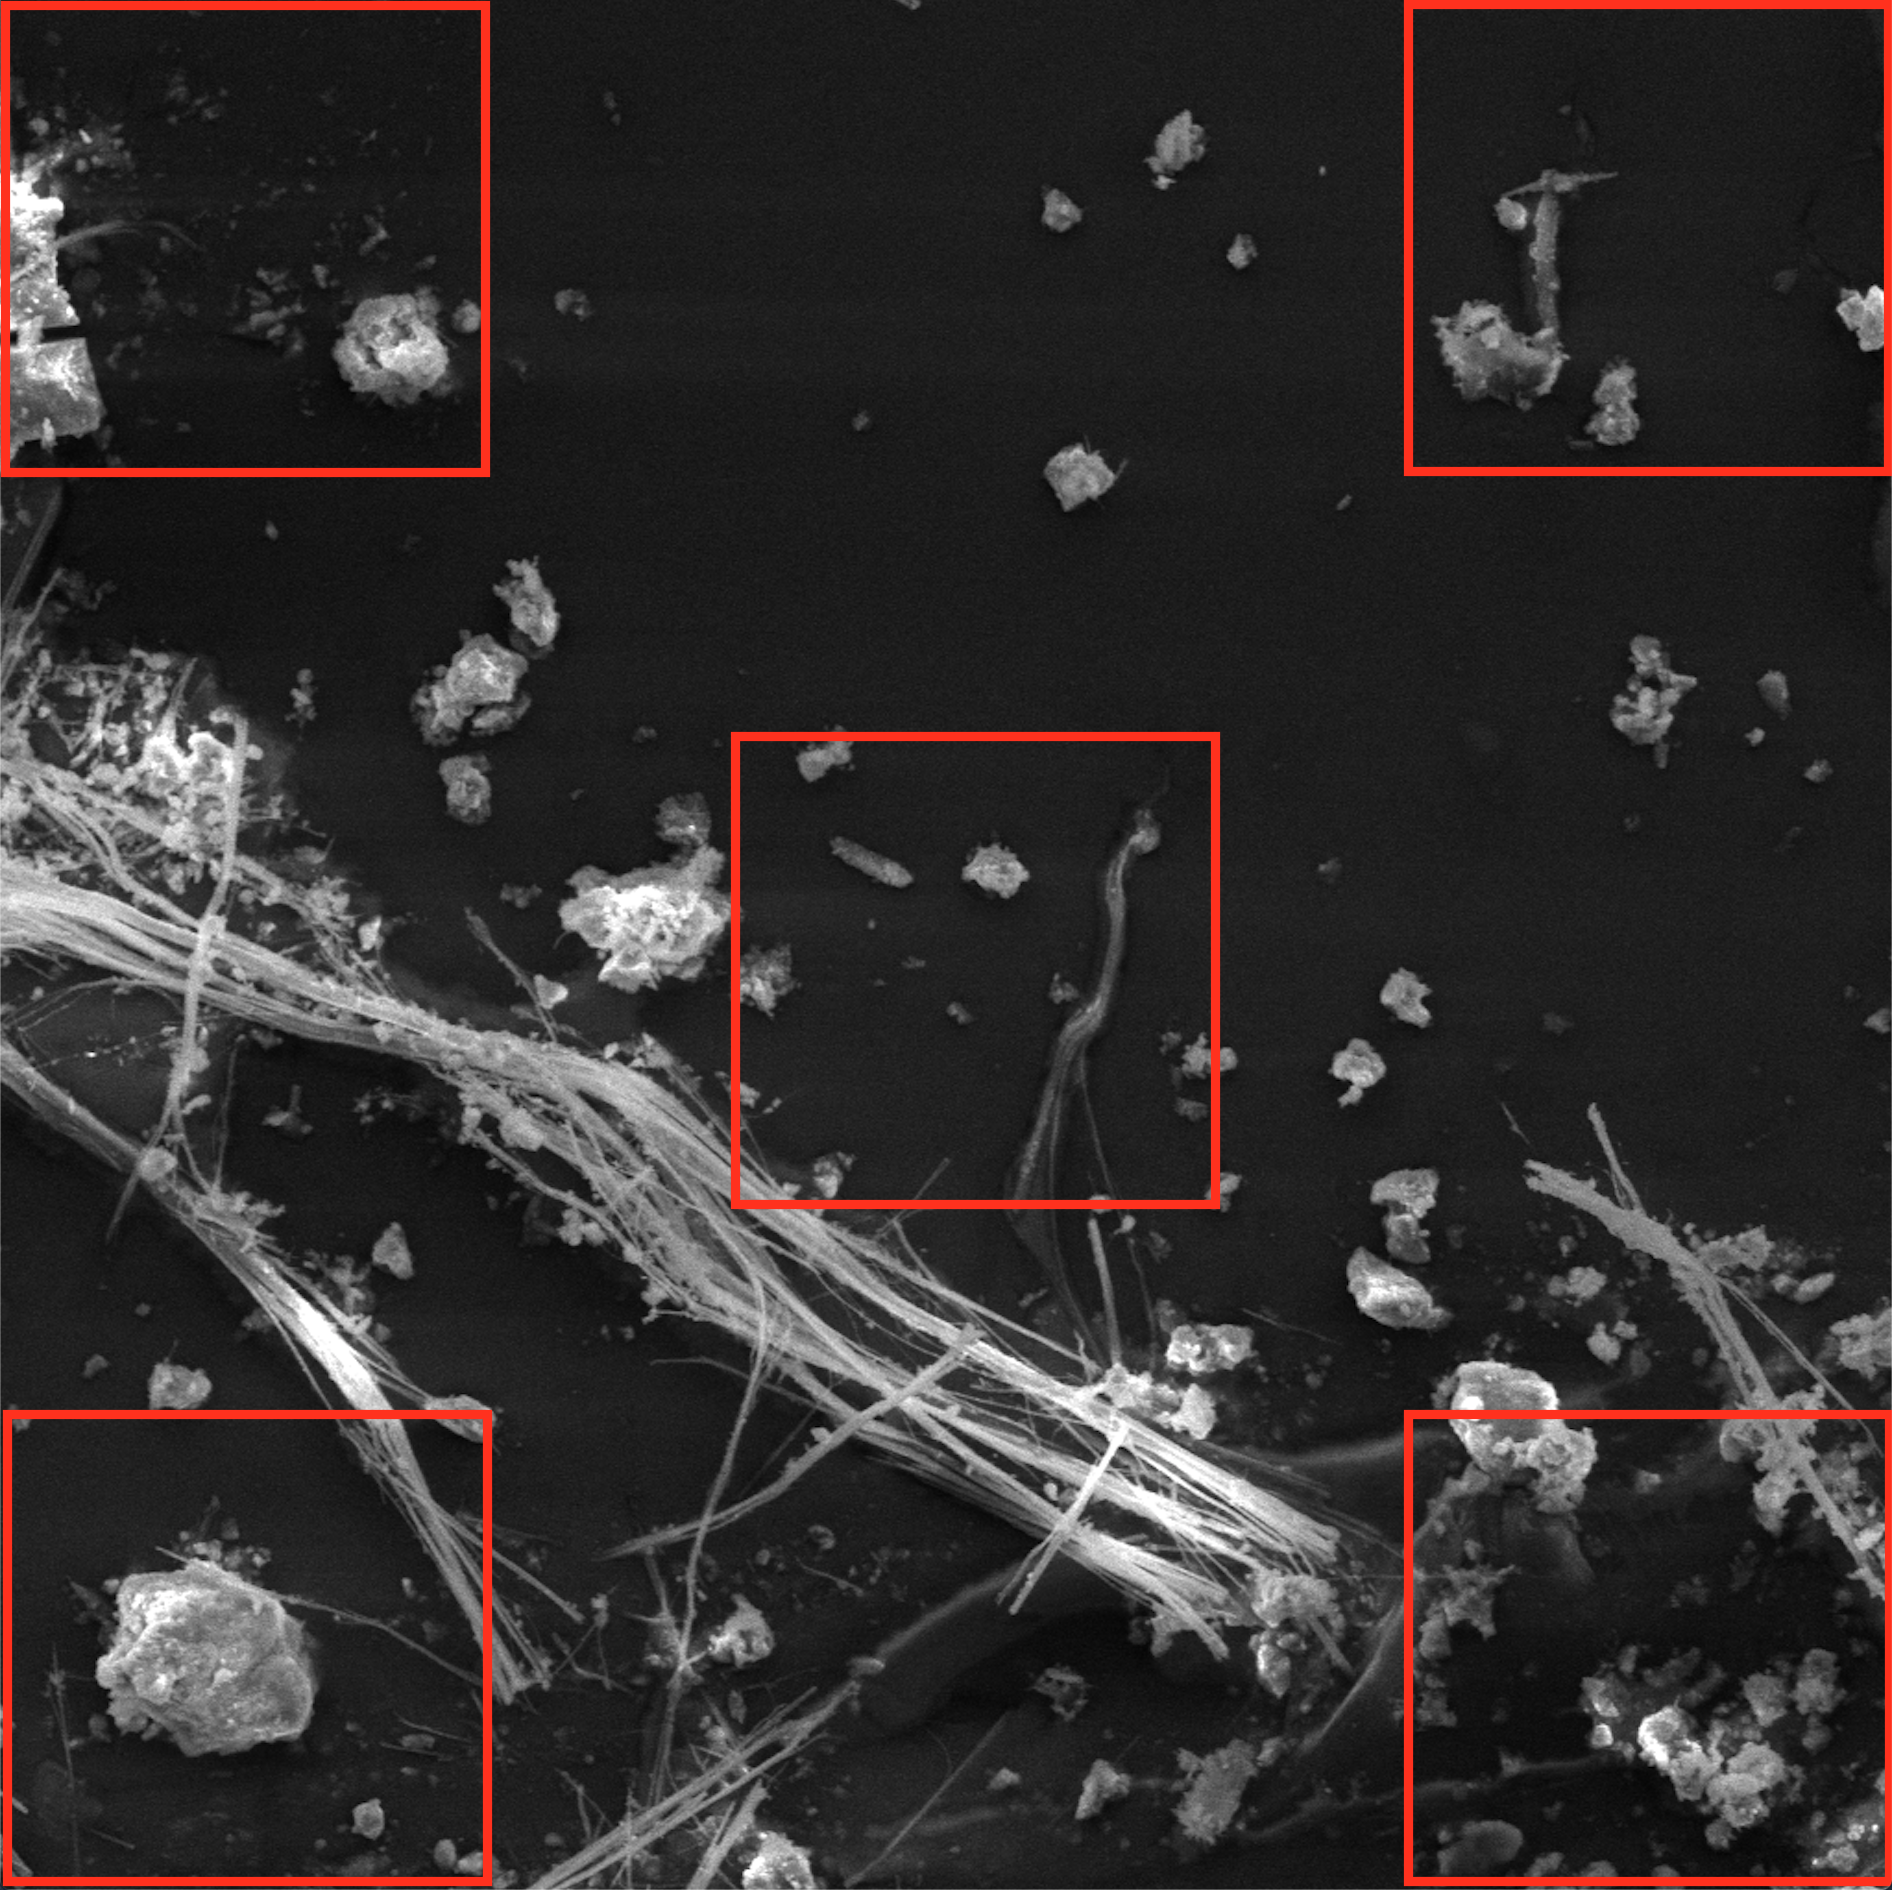
\includegraphics[scale=0.3]{chapter4/FiveCrop}
  \label{fig:FiveCrop}
\end{figure}

Possible fixes of the above mentioned problem are removing images that have asbestos spanning only part of the image, which would drastically reduce the image pool or devise another cropping method.

\subsection{RandomNine}

In order to mitigate the problem label preservation during cropping a new strategy has been implemented from scratch. The image is first randomly flipped horizontally with  a chance of 0.5, then it is randomly  flipped vertically with a chance of 0.5, then is it rotated by a random degree ranging from 0 to 359. After these transformations nine crops are taken from the image in a systematic way as seen in Figure \ref{fig:TenCrop}. This style of cropping does not resize the image thus does not lose potentially important information. I does however span roughly 60\% of the image and thus mitigates the problem of having wrong labels. I would argue that this cropping method with a dataset variation that  removes images where asbestos is only seen in a small, single area, should lead to better results.

\begin{figure}[H]
  \centering
  \caption{Own implementation of RandomNine after the image has been transformed.}
  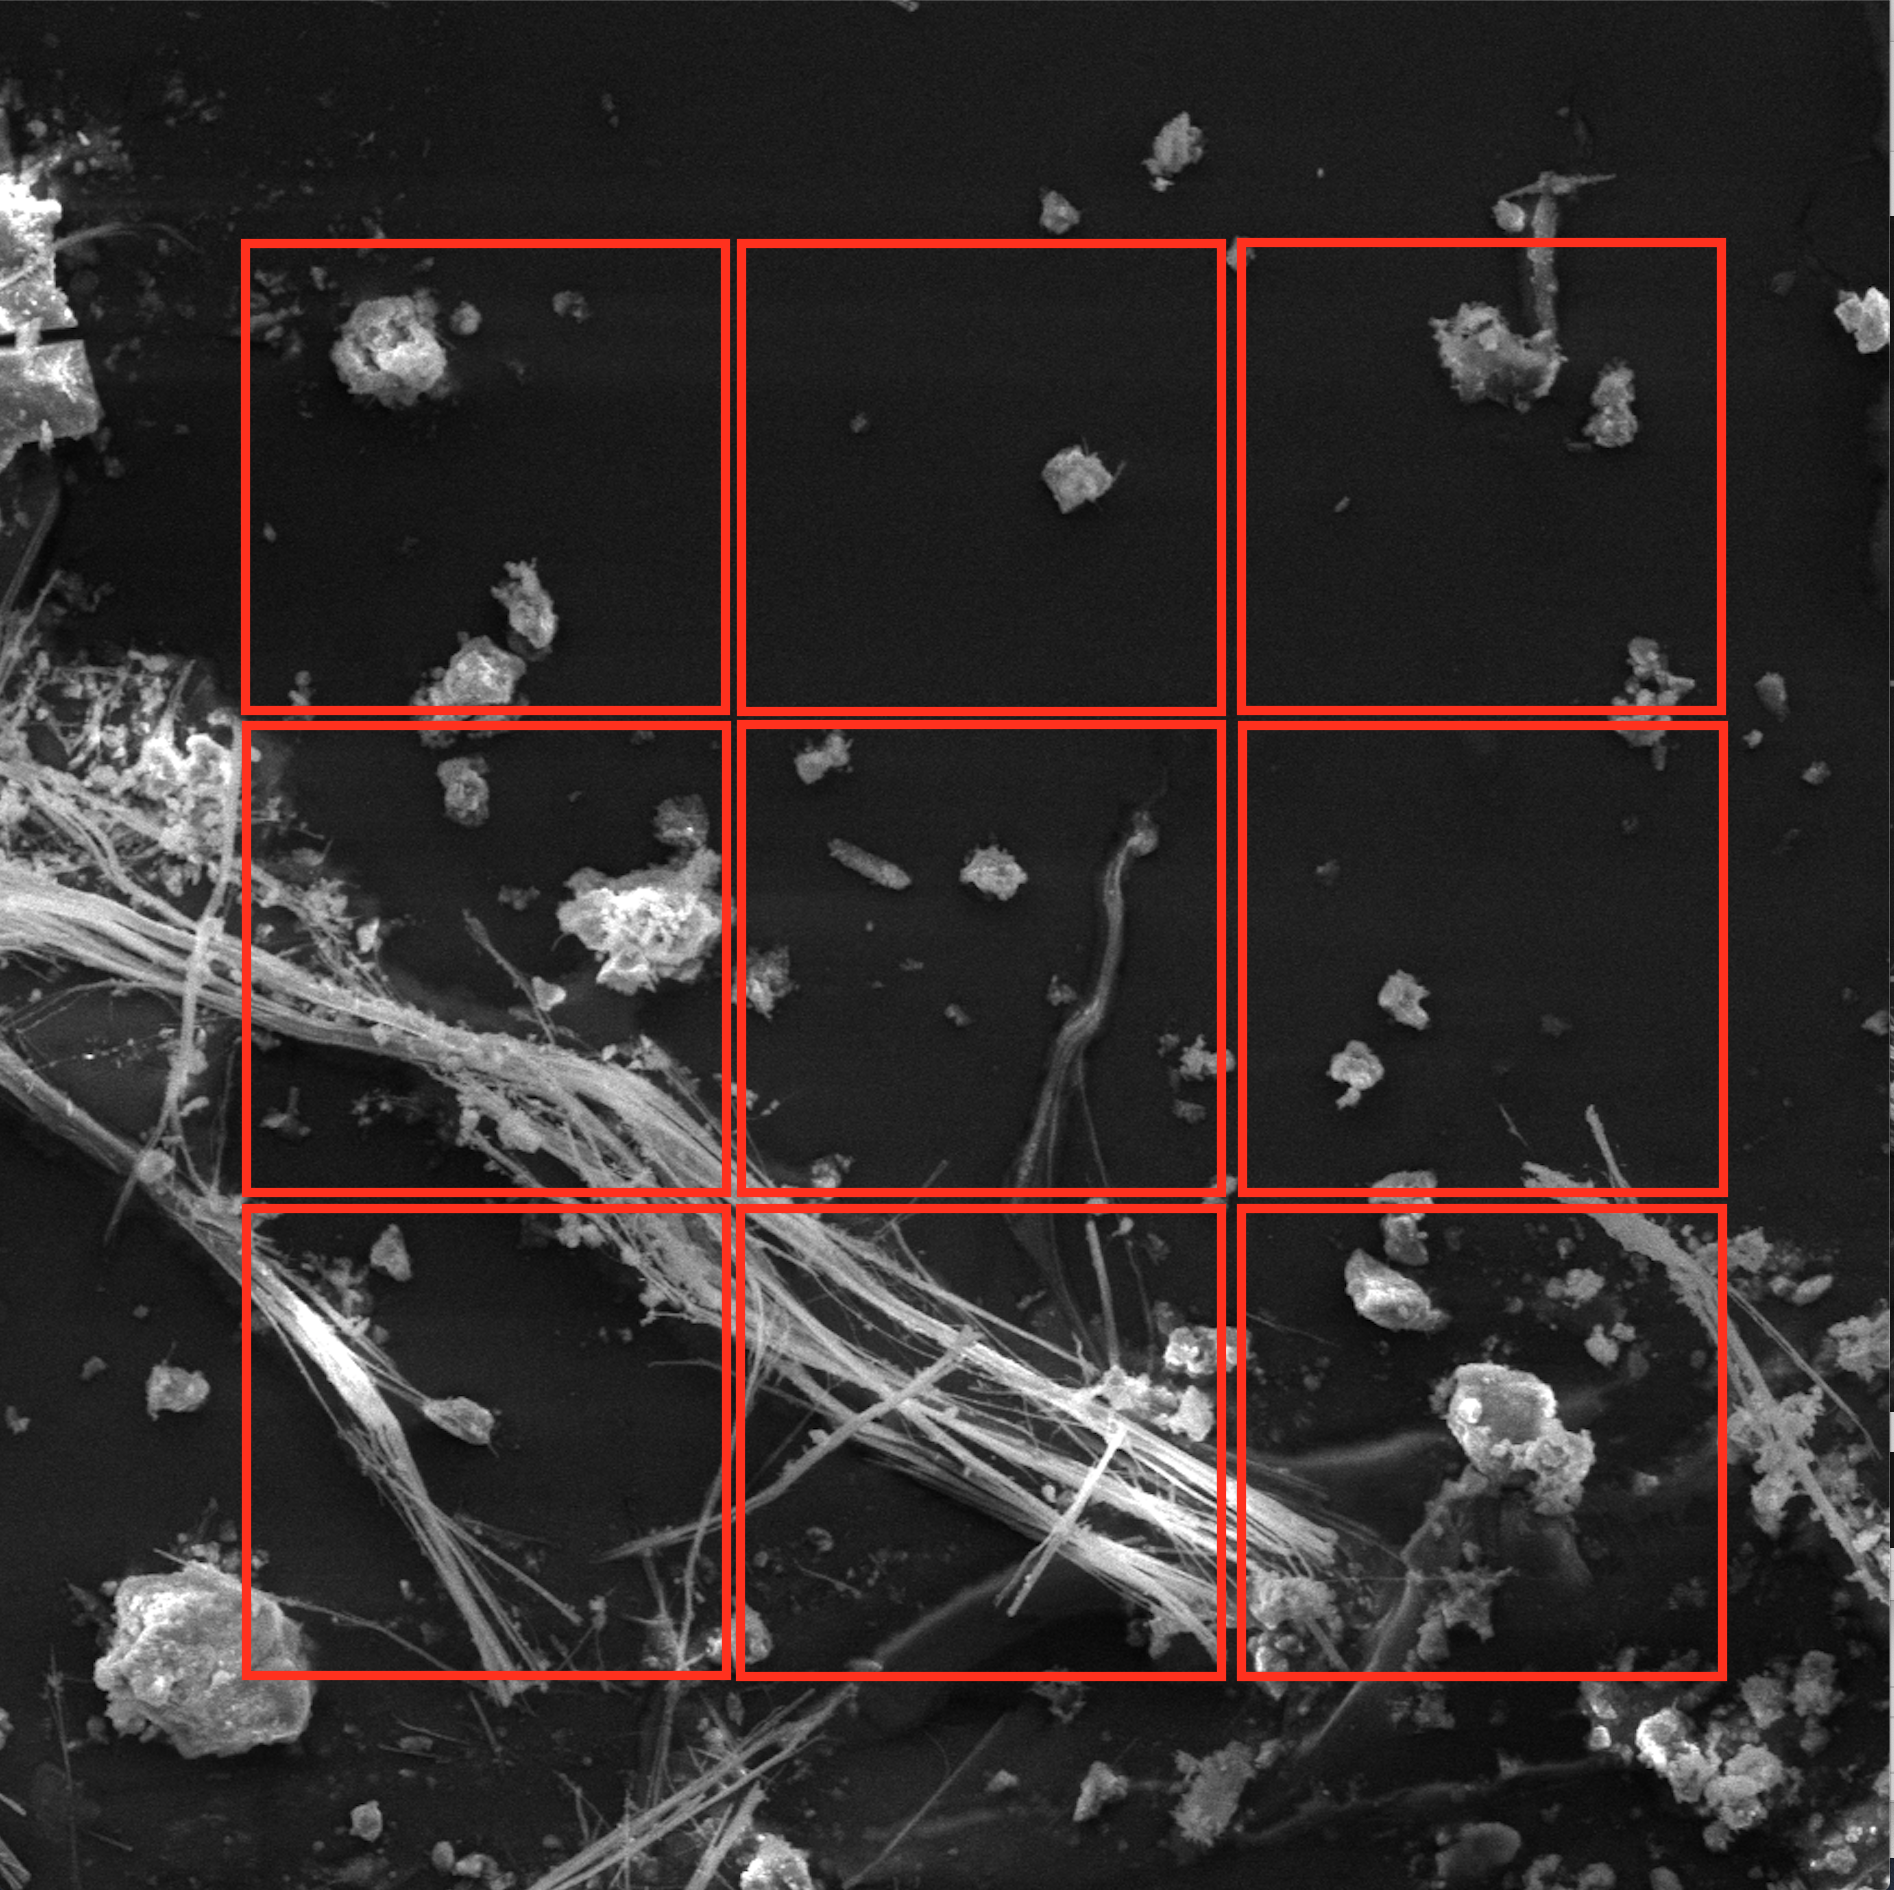
\includegraphics[scale=0.3]{chapter4/NineCrop}
  \label{fig:TenCrop}
\end{figure}


\section{ResNet18 modifications}

With the ResNet18 architecture I will pursue a similar approach as with VGG and reduce the filter size thus reducing the overall complexity of the model. I have decided define one variable that sets  the number of filters for every layer in  the architecture. This is done for  simplicity and because preliminary  experiments  have not shown any advantages to keep  the number of filters growing with the increasing depth of the network. I will reduce the  original amount of filter to 32 filters in a first run and then decrease them until only 1 filter remains per layer. \\

In a next step I will examine if changing the architecture in a way that accepts bigger input images leads to better results. The idea behind letting the network  accept bigger images it that  no or less re-sizing is  needed which destroys information in its process. The alterations are done in the first few layers where values like strike and kernel size can be changed, or new layers can be added that reduce the image size by a certain amount until the original input size of 224x224 pixels is reached. From that point on the unchanged ResNet18 architecture is used. In order to cope with the bigger images without running into memory overflow errors two strategies can be used.  The  first one is  to reduce the batch size which can  help to some extent but leads to greater overfitting and lower accuracies. The second one is to reduce the  parameters in  the network which is already done by reducing the number of filters. The second method allows for images to be processed in their full resolution with minimal memory consumption and without having to change the batch size.

\section{Conclusion}

In this chapter I laid down my thoughts on how to increase performance. First I will apply transfer learning on all architectures and their variants where present and compare the results. Then I will apply modifications to the architectures to see how fewer parameters and fewer filters perform. That has many benefits like smaller models, better deployability, faster learning and less overfitting. I will experiment with allowing ResNet18 to accept  bigger images without resizing them. Visualizing some  of the activation images and heatmaps should shed some light into what  actually is learned in the process.